\section{Gaseous Exchange and Respiration}

\begin{multicols}{2}


\section*{Gas Exchange in Mammals}


\subsection{Breathing Model} % VSO 34

\begin{center}
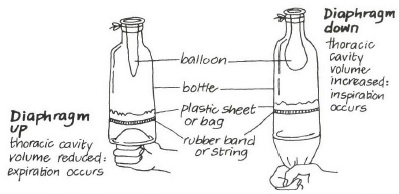
\includegraphics[width=0.49\textwidth]{./img/vso/breathing-model.jpg}
\end{center}

\begin{description*}
%\item[Subtopic:]{}
\item[Materials:]{Plastic bottle, balloons, plastic bag, string/rubber band, straw}
%\item[Setup:]{}
\item[Procedure:]{Cut the bottom off a plastic
bottle. Attach a balloon over the
bottle mouth so it hangs inside.
Fix a piece of plastic bag over the
cut base end using string or a rubber band. (Optional: Fix a straw through the bottle top and attach 1 or 2 balloons to the end inside the bottle.)}
%\item[Hazards:]{}
%\item[Questions:]{}
\item[Observations:]{Pulling the plastic bag down causes the balloon to inflate; pushing it up causes the balloon the deflate.}
\item[Theory:]{The balloon(s) represents the lung(s), the plastic bag the diaphragm, the bottle the thoracic cavity (and the straw the esophagus). Pulling the plastic sheet down causes an expansion of the cavity bringing about inspiration and causing the balloon to inflate. Pushing the sheet up reduces the volume of the cavity, causing expiration and the balloon to deflate.}
%\item[Applications:]{}
\item[Notes:]{Tell students that this model does not show the expansion and contraction of the rib cage with breathing.}
\end{description*}

\subsection{Gas Exchange Board Game}

\begin{center}
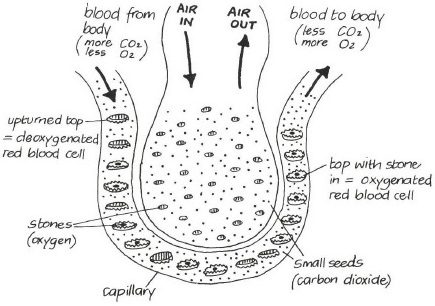
\includegraphics[width=0.49\textwidth]{./img/vso/gas-exchange-game.jpg}
\end{center}

\begin{description*}
%\item[Subtopic:]{}
\item[Materials:]{Large sheet of paper, bottle caps, seeds, stones}
%\item[Setup:]{}
\item[Procedure:]{Draw the capillary and alveolus as
shown. Students arrange the
stones (oxygen), seeds (carbon
dioxide) and bottle caps (red
blood cells) on the drawing. Colour the bottle caps red on the inside and blue on the outside.}
%\item[Hazards:]{}
%\item[Questions:]{}
%\item[Observations:]{}
\item[Theory:]{As the caps (red blood cells) enter the capillary most are turned to blue to show they contain no stone (oxygen). Stones are placed inside the alveolus which get moved into the capillary and transported away inside red upturned bottle caps (oxygenated red blood cells). The seeds (carbon dioxide) are moved from the capillary plasma area into the alveolus.}
%\item[Applications:]{}
%\item[Notes:]{}
\end{description*}

\subsection{Gas Exchange Game} % VSO 35

\begin{center}
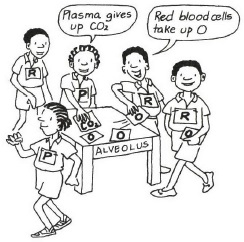
\includegraphics[width=0.4\textwidth]{./img/vso/gas-exchange-students.jpg}
\end{center}

\begin{description*}
%\item[Subtopic:]{}
\item[Materials:]{Cards, table}
%\item[Setup:]{}
\item[Procedure:]{The table represents the alveolus.
Students wear either an `R' or `P'
card and so act as red blood cells
(R) or plasma (P). When going
round the table the `R' students
pick up cards with `O'(oxygen)
on them. The `P' students put down the
`CO$_2$' (carbon dioxide) cards.}
%\item[Hazards:]{}
%\item[Questions:]{}
%\item[Observations:]{}
%\item[Theory:]{}
\item[Applications:]{Link this activity with \nameref{sub:circulation-game} (p.~\pageref{sub:circulation-game}).}
%\item[Notes:]{}
\end{description*}

%==================================================================================================%

\section*{Gas Exchange in Plants}


\subsection{Germinating Seeds} % Source 113

\begin{center}
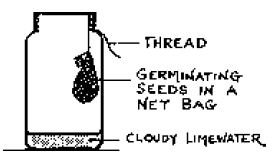
\includegraphics[width=0.4\textwidth]{./img/source/germinating-seeds.png}
\end{center}

\begin{description*}
%\item[Subtopic:]{}
\item[Materials:]{Glass jar, limewater, plastic bag, peas}
%\item[Setup:]{}
\item[Procedure:]{Put a little lime water into a wide-mouthed glass jar and hang a perforated plastic bag,
containing soaked and germinating peas. Make sure that the peas are separated from the
liquid. Seal the jar well and leave it to stand for a few hours.}
%\item[Hazards:]{}
%\item[Questions:]{}
\item[Observations:]{The limewater becomes cloudy.}
\item[Theory:]{The germinating peas respire giving out carbon dioxide.}
%\item[Applications:]{}
%\item[Notes:]{}
\end{description*}

%==================================================================================================%

\section*{Respiration}


\subsection{Respiration Cards} % VSO 36

\begin{center}
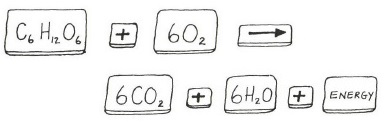
\includegraphics[width=0.49\textwidth]{./img/vso/respiration-cards.jpg}
\end{center}

\begin{description*}
%\item[Subtopic:]{}
\item[Materials:]{Cards}
%\item[Setup:]{}
\item[Procedure:]{Cut out cards to represent the substances involved in respiration. Label
some cards with a `+' or an arrow. Mix up the cards and ask students to
arrange them correctly as shown.}
%\item[Hazards:]{}
%\item[Questions:]{}
%\item[Observations:]{}
%\item[Theory:]{}
%\item[Applications:]{}
%\item[Notes:]{}
\end{description*}

\subsection{Respiration Plates}

\begin{center}
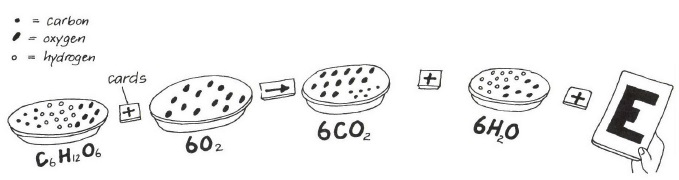
\includegraphics[width=0.49\textwidth]{./img/vso/respiration-plates.jpg}
\end{center}

\begin{description*}
%\item[Subtopic:]{}
\item[Materials:]{Various seeds, bottle caps, coins, etc., plates, card}
%\item[Setup:]{}
\item[Procedure:]{Choose 3 different types of seed, coin or bottle cap to represent carbon,
hydrogen and oxygen. Arrange 4 plates or boxes on a table as shown.
Ask students to place the correct number of seeds etc. on the plates.
When the seeds are placed correctly the card carrying the `E' for energy
is added.}
%\item[Hazards:]{}
%\item[Questions:]{}
%\item[Observations:]{}
%\item[Theory:]{}
\item[Applications:]{Demonstrate that the reverse equation is the process of
photosynthesis.}
%\item[Notes:]{}
\end{description*}

\subsection{Exhaling $\mathrm{CO_2}$} % VSO 34 Shika 107

\begin{center}
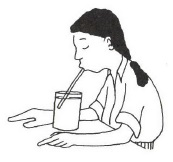
\includegraphics[width=0.4\textwidth]{./img/vso/exhale-co2.jpg}
\end{center}

\begin{description*}
%\item[Subtopic:]{}
\item[Materials:]{Straw or pen tube, limewater}
%\item[Setup:]{}
\item[Procedure:]{Breathe out through a straw or the barrel of a ball point pen into filtered limewater.}
%\item[Hazards:]{}
%\item[Questions:]{}
\item[Observations:]{The limewater goes cloudy then later clear.}
\item[Theory:]{The exhaled carbon dioxide reacts with the calcium hydroxide solution (lime water) making a precipitation, which later dissolves by more carbon dioxide to soluble calcium hydrogen
carbonate.}
%\item[Applications:]{}
%\item[Notes:]{}
\end{description*}

\subsection{Yeast Balloons} % Shika 221 PIC!!!

%\begin{center}
%\includegraphics[width=0.4\textwidth]{./img/.png}
%\end{center}

\begin{description*}
%\item[Subtopic:]{}
\item[Materials:]{Bottle, balloon, warm water, sugar, yeast}
%\item[Setup:]{}
\item[Procedure:]{Fill a bottle partly with a warm water/sugar solution. Add a small amount of yeast into a balloon. Stretch the mouth of the balloon over the bottle, then lift the balloon to empty its contents into the bottle.}
%\item[Hazards:]{}
%\item[Questions:]{}
\item[Observations:]{After a few hours, the balloon inflates.}
\item[Theory:]{Yeast is a an organism that eats sugar and breaks it down into alcohols and carbon dioxide. The carbon dioxide gets collected in the balloon.}
\item[Applications:]{This process is the basis for making beers, wines and other alcoholic beverages.}
%\item[Notes:]{}
\end{description*}

\subsection{Fermenting Fruits} % Source 114

\begin{center}
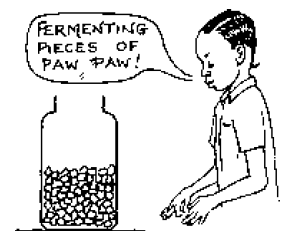
\includegraphics[width=0.4\textwidth]{./img/source/fermenting-fruits.png}
\end{center}

\begin{description*}
%\item[Subtopic:]{}
\item[Materials:]{Fruit pulp (e.g. pawpaw), sugar, water, container}
%\item[Setup:]{}
\item[Procedure:]{Prepare a pulp of paw paw. Put the pulp into a glass. Let it stand for some time in a warm
place.}
%\item[Hazards:]{}
%\item[Questions:]{}
\item[Observations:]{Gas bubbles are formed in the pulp}
\item[Theory:]{The pulp is fermented because the sugar contained in it is acted on by wild yeast, which
grows on the skin of the fruit. Yeasts are also found in air.}
\item[Applications:]{Making local brews (e.g. pombe)}
%\item[Notes:]{}
\end{description*}


\end{multicols}

\pagebreak